\documentclass[12pt]{article}

%font
\usepackage{mathptmx}


%spacing
\usepackage{setspace}
\doublespacing

%pages
\usepackage[paperheight=11in,paperwidth=8.5in,margin=1in]{geometry}


\usepackage{todonotes}
\newcommand{\pe}[1]{\todo[inline, backgroundcolor=green]{PE: #1}}
\definecolor{eyecancerpink}{rgb}{1.0, 0.0, 1.0}
\newcommand{\nm}[1]{\todo[inline, backgroundcolor=eyecancerpink]{NM: #1}}

\usepackage{cite}
\usepackage{amsmath,amssymb,amsfonts}
\usepackage{algorithmic}
\usepackage{graphicx}
\usepackage{textcomp}
\usepackage{xcolor}
\usepackage{tikz}
\usepackage{hyperref}
\usepackage{float}
\usepackage{multicol}
\usepackage{caption}
\usepackage{subcaption}
\usepackage{enumitem}


\author{Nicola J. Müller, Robert Leist, Paul Eichler, \\and Tobias Recktenwald}
\title{Towards Language Model-based Identification of Market Segments and Fostering of Business Clusters}

\begin{document}
    \maketitle
   \begin{abstract}
   	Identifying market segments is crucial for effective marketing strategies and well-informed business decisions. Further, combining companies' geographical locations with their market segments allows for detecting business clusters. However, acquiring and processing the data needed to gain such insights into regional economies is labor-intensive. 
   	
   	We propose to circumvent these challenges by leveraging state-of-the-art language models to transform companies' highly informative public text data into low-dimensional vectors and then applying clustering to identify market segments and make location recommendations for novel companies to support business cluster development. 
   	
   	A qualitative evaluation of our methods being applied to data from the German municipality Saarland demonstrates that our methods can accurately cluster similar companies and assign novel companies to existing clusters.
   \end{abstract}
   
   
   \section{Introduction}
   Deciding on the location of a business is a vital strategic decision: First, most businesses must be located close to their customers and suppliers for more effective marketing or reduced transportation costs. Secondly, being located in an active regional cluster can significantly benefit business growth \cite{clustersandcomp,gems-model, regionaladv, clustertheory}. 
   
   Business clusters are local concentrations of companies, manufacturers, suppliers, and institutions from the same field. Identifying clusters combines geographical data of companies' locations with information on their corresponding market segments. This proximity of related companies enables efficient cooperation and knowledge transfer, which has been shown to significantly increase the productivity of all companies within the cluster \cite{clustersandcomp,gems-model, regionaladv, clustertheory}. Thus, establishing or further developing business clusters is of high interest to companies and local governments. Therefore, significant effort is spent identifying clusters and market segments in regional economies. 
   
   However, identifying market segments and business clusters requires a significant amount of manual labor. Typically, one must first collect information about companies in the targeted region. Afterward, for each company, their publicly available information must be analyzed to understand their products, strategic position, market positioning, and further characteristics. 
   This process is labor-intensive, as businesses do not provide specific data on the latter points, but it must be inferred from their product portfolio and websites. Additionally, even basic data like the number of employees is often unavailable or difficult to collect automatically, especially for small regional companies.
   At the same time, recent advances in natural language processing (NLP), e.g., the popular ChatGPT \cite{chatgpt}, have yielded surprisingly good results in numerous applications. Especially they have proven to be very efficient at extracting data and summaries from human written texts.
   
   The main contribution of this work is an automatic clustering pipeline to identify market segments and business clusters from publicly available information. Additionally, our system can utilize the found clusters to provide strategic location recommendations, which we will demonstrate using the German federal state Saarland as an example. The novelty of our approach is that we rely on language models to process the companies' information, allowing us to circumvent many of the challenges attributed to gathering economic data. 
   Our clustering pipeline can be divided into $4$ distinct steps: $1)$ gathering descriptions from the websites of companies in the region of interest, $2)$ computing embeddings of the text data, $3)$ reducing the embeddings' dimensionality, and $4)$ applying clustering algorithms.
   Our location recommendation system builds upon the clustering pipeline by computing an embedding of a novel company's description, assigning it to a cluster, and then identifying the most similar companies within the cluster. The system then recommends that the novel company locate its site near an established company acting in the same market segment, which fosters business cluster development.
   We provide a graphical user-interface for our methods, which visualizes the clustering of companies and their locations in an interactive manner, allowing end-users to analyze the various predicted market segments. Further, the interface supports making location recommendations for new company sites using text inputs.
   
   In summary, our main contributions are:
   \begin{itemize}[noitemsep]
   	\item Circumventing the challenges of economic data collection by relying on public text data.
   	\item Leveraging state-of-the-art language models to apply clustering algorithms to text data.
   	\item Showing how our methods can be extended to handle additional features.
   	\item Demonstrating our approach's feasibility using Saarland's economy and providing a user-friendly graphical interface.
   \end{itemize}
   
   \section{Related Work}
   This section will examine previous work on business clusters and recent advances in natural language processing.
   
   Business clusters and their advantages have been studied in many works. For example, \cite{regionaladv} examined the well-known technology cluster in Silicon Valley, famous for being the home of many innovative start-ups. 
   \cite{clustertheory} provides a detailed discussion of the cluster phenomenon. It discusses preexisting literature on clusters and reviews the main positive effects commonly observed in clusters, positive feedback and productivity \& growth. Additionally, it provides examples of well-known clusters.
   
   The region of choice for testing our approach, Saarland, has also been the subject of scientific work. It should be noted that Saarland is mostly investigated for its location on the border of France and Luxembourg or because of its mining and steel-producing past.
   These factors are, however, of no interest to this work. For example, \cite{saarlandeco1} has focused on the agglomeration of the automotive industry in Saarland and the neighboring regions but focuses on the challenges that the country borders pose to this industry.
   The paper \cite{saarlandeco2} specifically compares the economic strategies for developing the region's economy with a focus on how clusters are developed. Most importantly, they identify some regional business clusters. We will revisit these when evaluating our clustering algorithm and compare the clusters and market segments identified by our approach. It should be noted, however, that the paper was published in 2009, meaning their analysis could be outdated to some extent.
   
   In natural language processing (NLP), translating text data to machine-processable representations is a fundamental challenge for numerous tasks, such as sentiment analysis~\cite{rezaeinia2019sentiment}, and information retrieval~\cite{ye2016word}, due to the complexity and variability of natural language. A popular approach for representing text data is the utilization of so-called \emph{embeddings}: vectorized representations of text with the property that vectors of text data with similar semantic and syntactic properties will have a smaller distance to vectors of text data with different properties, making them ideal for applying clustering to our sparse dataset of high-dimensional company descriptions.  
   Mikolov et al~\cite{mikolov2013efficient}. popularized learning word embeddings from raw text data in $2013$ by introducing their Word2Vec model. More recently, transformer-based models like BERT, developed by Devlin et al.~\cite{devlin2018bert}, and GPT models by OpenAI~\cite{radford2018improving, chatgpt} have leveraged context-dependent word embeddings by encoding the words themselves and the context in which they are used. So-called sentence transformers extended these approaches by computing embeddings for entire sentences to capture more contextual information than individual word embeddings. Reimers and Gurevych~\cite{reimers2019sentence} introduced the Sentence-BERT model, capable of generating high-quality sentence embeddings using only a fraction of the original BERT model's computational effort.
   
   \section{Procedure}
   \begin{figure}[H]
    \centering
    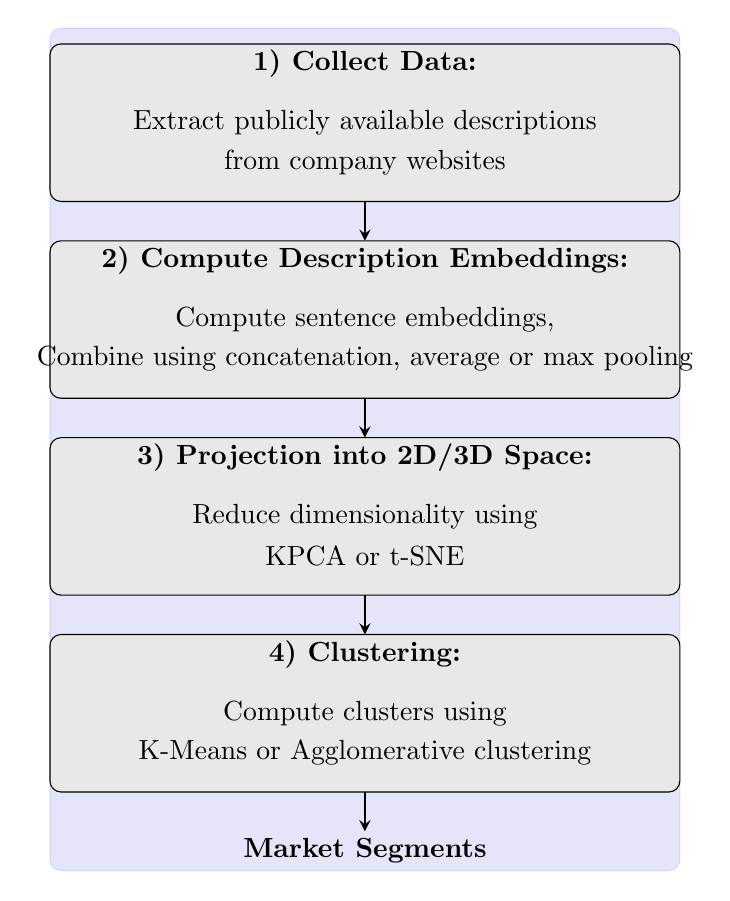
\begin{tikzpicture}
        \definecolor{lightgrey}{RGB}{232,232,232}
        \definecolor{darkblue}{RGB}{0,0,204}
        
        \draw[rounded corners, darkblue, fill=darkblue, opacity=0.1] (-4, -1) rectangle (4, 9.7);
    
        \draw[rounded corners, fill=lightgrey] (-4,7.5) rectangle (4, 9.5);
        \node[font=\bfseries] at (0, 9.25) {1) Collect Data:};
        \node at (0, 8.5) {Extract publicly available descriptions};
        \node at (0, 8.0) {from company websites};
        \draw[thick, -stealth] (0, 7.5) -- (0, 7);
    
        \draw[rounded corners, fill=lightgrey] (-4,5) rectangle (4, 7);
        \node[font=\bfseries] at (0, 6.75) {2) Compute Description Embeddings:};
        \node at (0, 6) {Compute sentence embeddings,};
        \node at (0, 5.5) {Combine using concatenation, average or max pooling};
        \draw[thick, -stealth] (0, 5) -- (0, 4.5);

        \draw[rounded corners, fill=lightgrey] (-4,2.5) rectangle (4, 4.5);
        \node[font=\bfseries] at (0, 4.25) {3) Projection into 2D/3D Space:};
        \node at (0, 3.5) {Reduce dimensionality using};
        \node at (0, 3.0) {KPCA or t-SNE};
        \draw[thick, -stealth] (0, 2.5) -- (0, 2);

        
        \draw[rounded corners, fill=lightgrey] (-4,0) rectangle (4, 2);
        \node[font=\bfseries] at (0, 1.75) {4) Clustering:};
        \node at (0, 1) {Compute clusters using};
        \node at (0, 0.5) {K-Means or Agglomerative clustering};
        \draw[thick, -stealth] (0, 0) -- (0, -0.5); 

        \node[font=\bfseries] at (0, -0.75) {Market Segments};
    \end{tikzpicture}
    \caption{Overview of our clustering pipeline.}
    \label{fig:pipeline}
\end{figure}
\pe{ s/Market Segments/Local Clusters; Market segment seems to be defined as segmenting your customer base \href{https://en.wikipedia.org/wiki/Market_segmentation}{wiki market segmentation}}


   Our goal is to collect data points on companies in the region of interest and cluster them to identify market segments and recommend locations for companies who plan to establish new sites, such that it supports the development of business clusters. We will present our clustering pipeline and then examine how we can use the results to provide location recommendations. 
   
   Figure \ref{fig:pipeline} shows a graphical representation of our general clustering pipeline, consisting of $4$ steps: $1)$ Collection of company descriptions, $2)$ computing embeddings, $3)$ reducing the embeddings' dimensionality, and $4)$ applying a clustering algorithm. In the following, we will examine each of these steps in detail.
   
   \textit{$1)$ Collect Descriptions:} The traditional approach for building an economic dataset would be to gather several attributes, like revenue, number of employers, and products, for many companies in the region of interest and then store each in a fixed-size vector. However, it is generally unclear which are the best attributes for representing companies. Further, encoding non-numerical attributes, like products and customer base, so that clustering algorithms can parse them is not straightforward. 
   Lastly, some attributes may be unavailable for some companies, meaning we would need to discard them or we would need to insert dummy values, which could lead to unwanted effects.
   To address these challenges to dataset construction, we propose representing companies by the description on their websites instead of numerical attributes. The benefit of using this data is that, since companies design their website to attract customers and investors, they include the most relevant information. Hence, we circumvent the problem of creating a targeted aggregator for specific information, making our approach simpler to implement and significantly more scalable \& automatable for larger target regions. 
   
   \textit{$2)$ Compute Embeddings:} To achieve the fixed-size inputs, we map each company description to an embedding that describes the data in a low-dimensional space. We rely on a sentence transformer model to compute embeddings for each sentence in a company's description. We then attain a single embedding for each description by taking the maximum over each feature dimension, which we denote as max pooling.
   
   \textit{$3)$ Projection into 2D Space:} The embeddings' number of features might be too large relative to the size of the dataset, potentially invoking the curse of dimensionality~\cite{koppen2000curse}. Further, clustering data in high-dimensional space prevents visualizing the results. Hence, we project the embeddings to 2D space. To do so, we apply the \emph{t-distributed stochastic neighbor embedding} (t-SNE) technique, which computes a probability distribution representing the pairwise similarity between data points in the feature space and then projects the data points to a low-dimensional space according to a second probability distribution that minimizes the Kullback-Leibler divergence to the first distribution. This enables t-SNE to accurately preserve local structures in the data, making it suitable for identifying clusters.
   
   \textit{$4)$ Clustering:} We cluster the data using agglomerative clustering, which initially assigns each data point to a separate cluster and then iteratively merges close clusters until all data points are in the same cluster. The intermediate clustering that achieves the largest separation between data points is chosen as the final clustering.
   Once the algorithm converges, we receive cluster labels for each company in our dataset, allowing us to infer market segments.
   
   Although our general pipeline represents companies using their descriptions, we emphasize that our approach can also utilize additional features. For instance, we can include the companies' products in the encoding by computing the corresponding sentence embeddings and merging them with the description embedding using max pooling.
   
   Figure \ref{fig:clustering-analysis} depicts the clustering analysis tab of our user-interface. On the left side, users can define how the description embeddings are computed, the technique and target dimensionality of the dimensionality reduction, and the number of clusters. Additionally, users can specify a subset of additional features, including industry, products, customer base, market positioning, and revenue, which will be combined with the descriptions. After clicking "Compute clustering", the clustered data points are shown on the right side. Further, users can see the location and clustering assignment of all companies in the given dataset on a map. When hovering the mouse over a company's data point, additional information about the company is shown.
   
   \begin{figure}[H]
   	\centering
   	\begin{subfigure}[b]{0.48\textwidth}
   		\centering
   		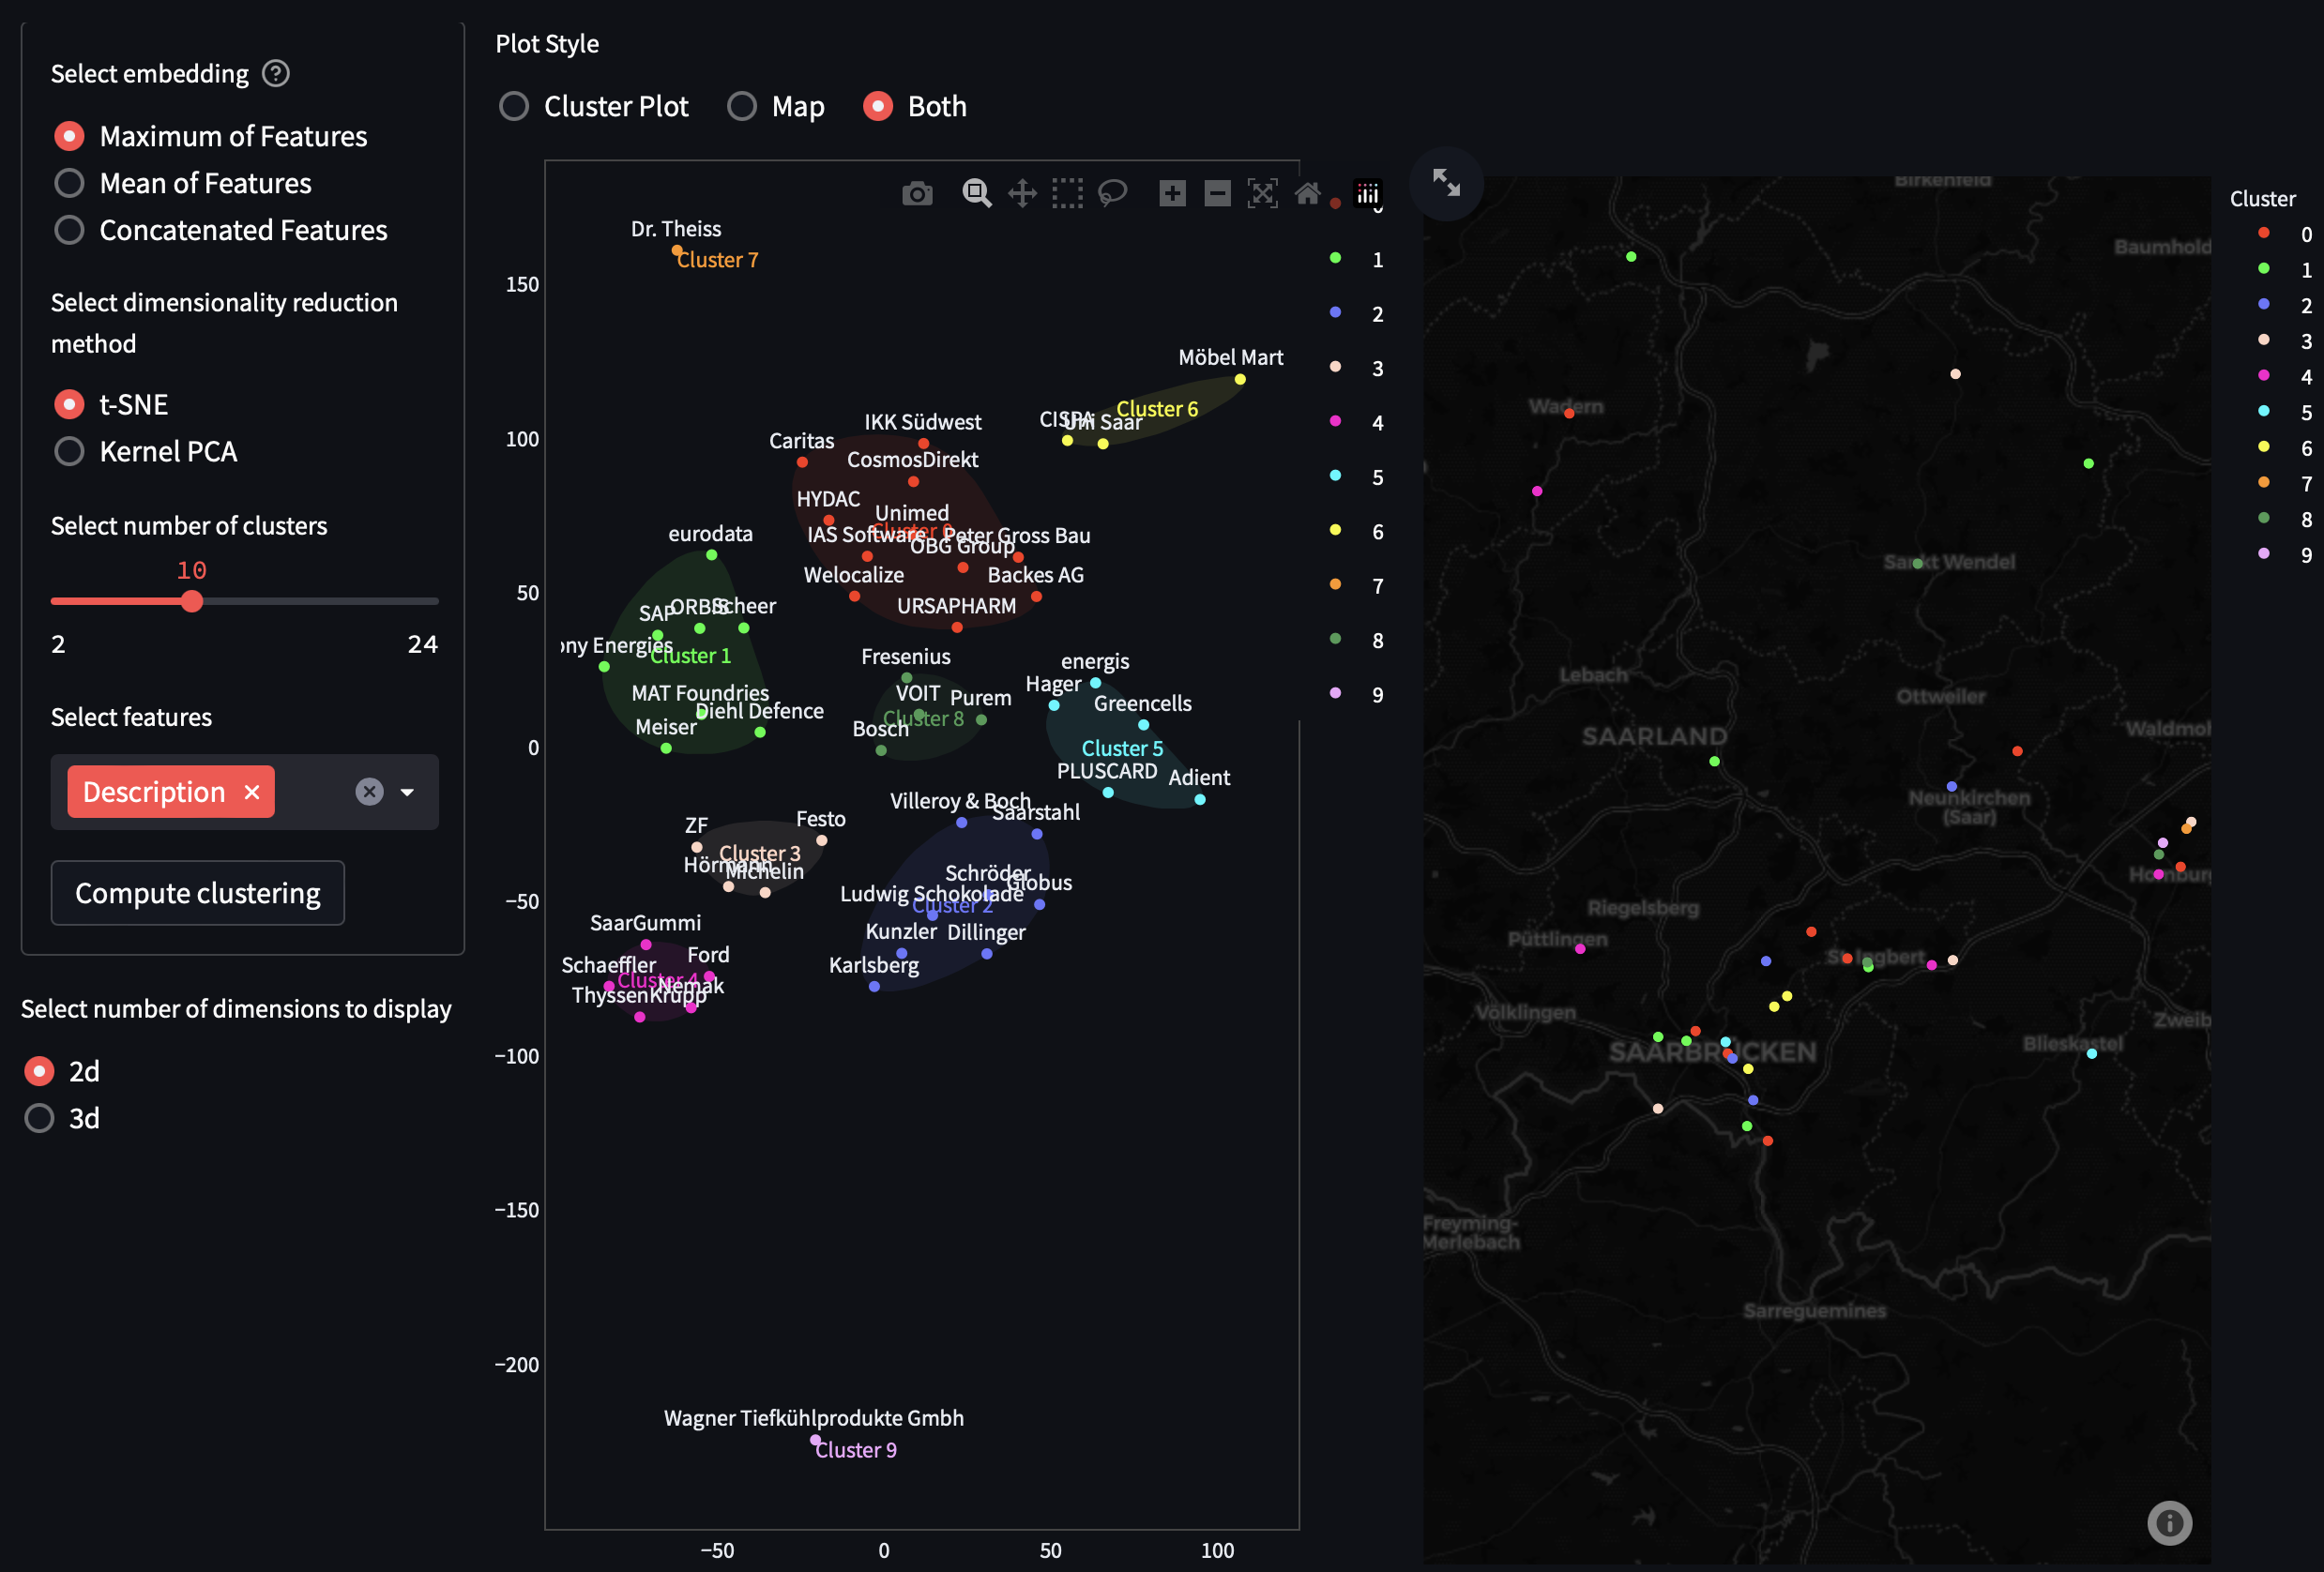
\includegraphics[width=\textwidth]{figures/clustering_analysis.png}
   		\caption{Clustering analysis page of our user-interface.}
   		\label{fig:clustering-analysis}
   	\end{subfigure}
   	\hfil
   	\begin{subfigure}[b]{0.48\textwidth}
   		\centering
   		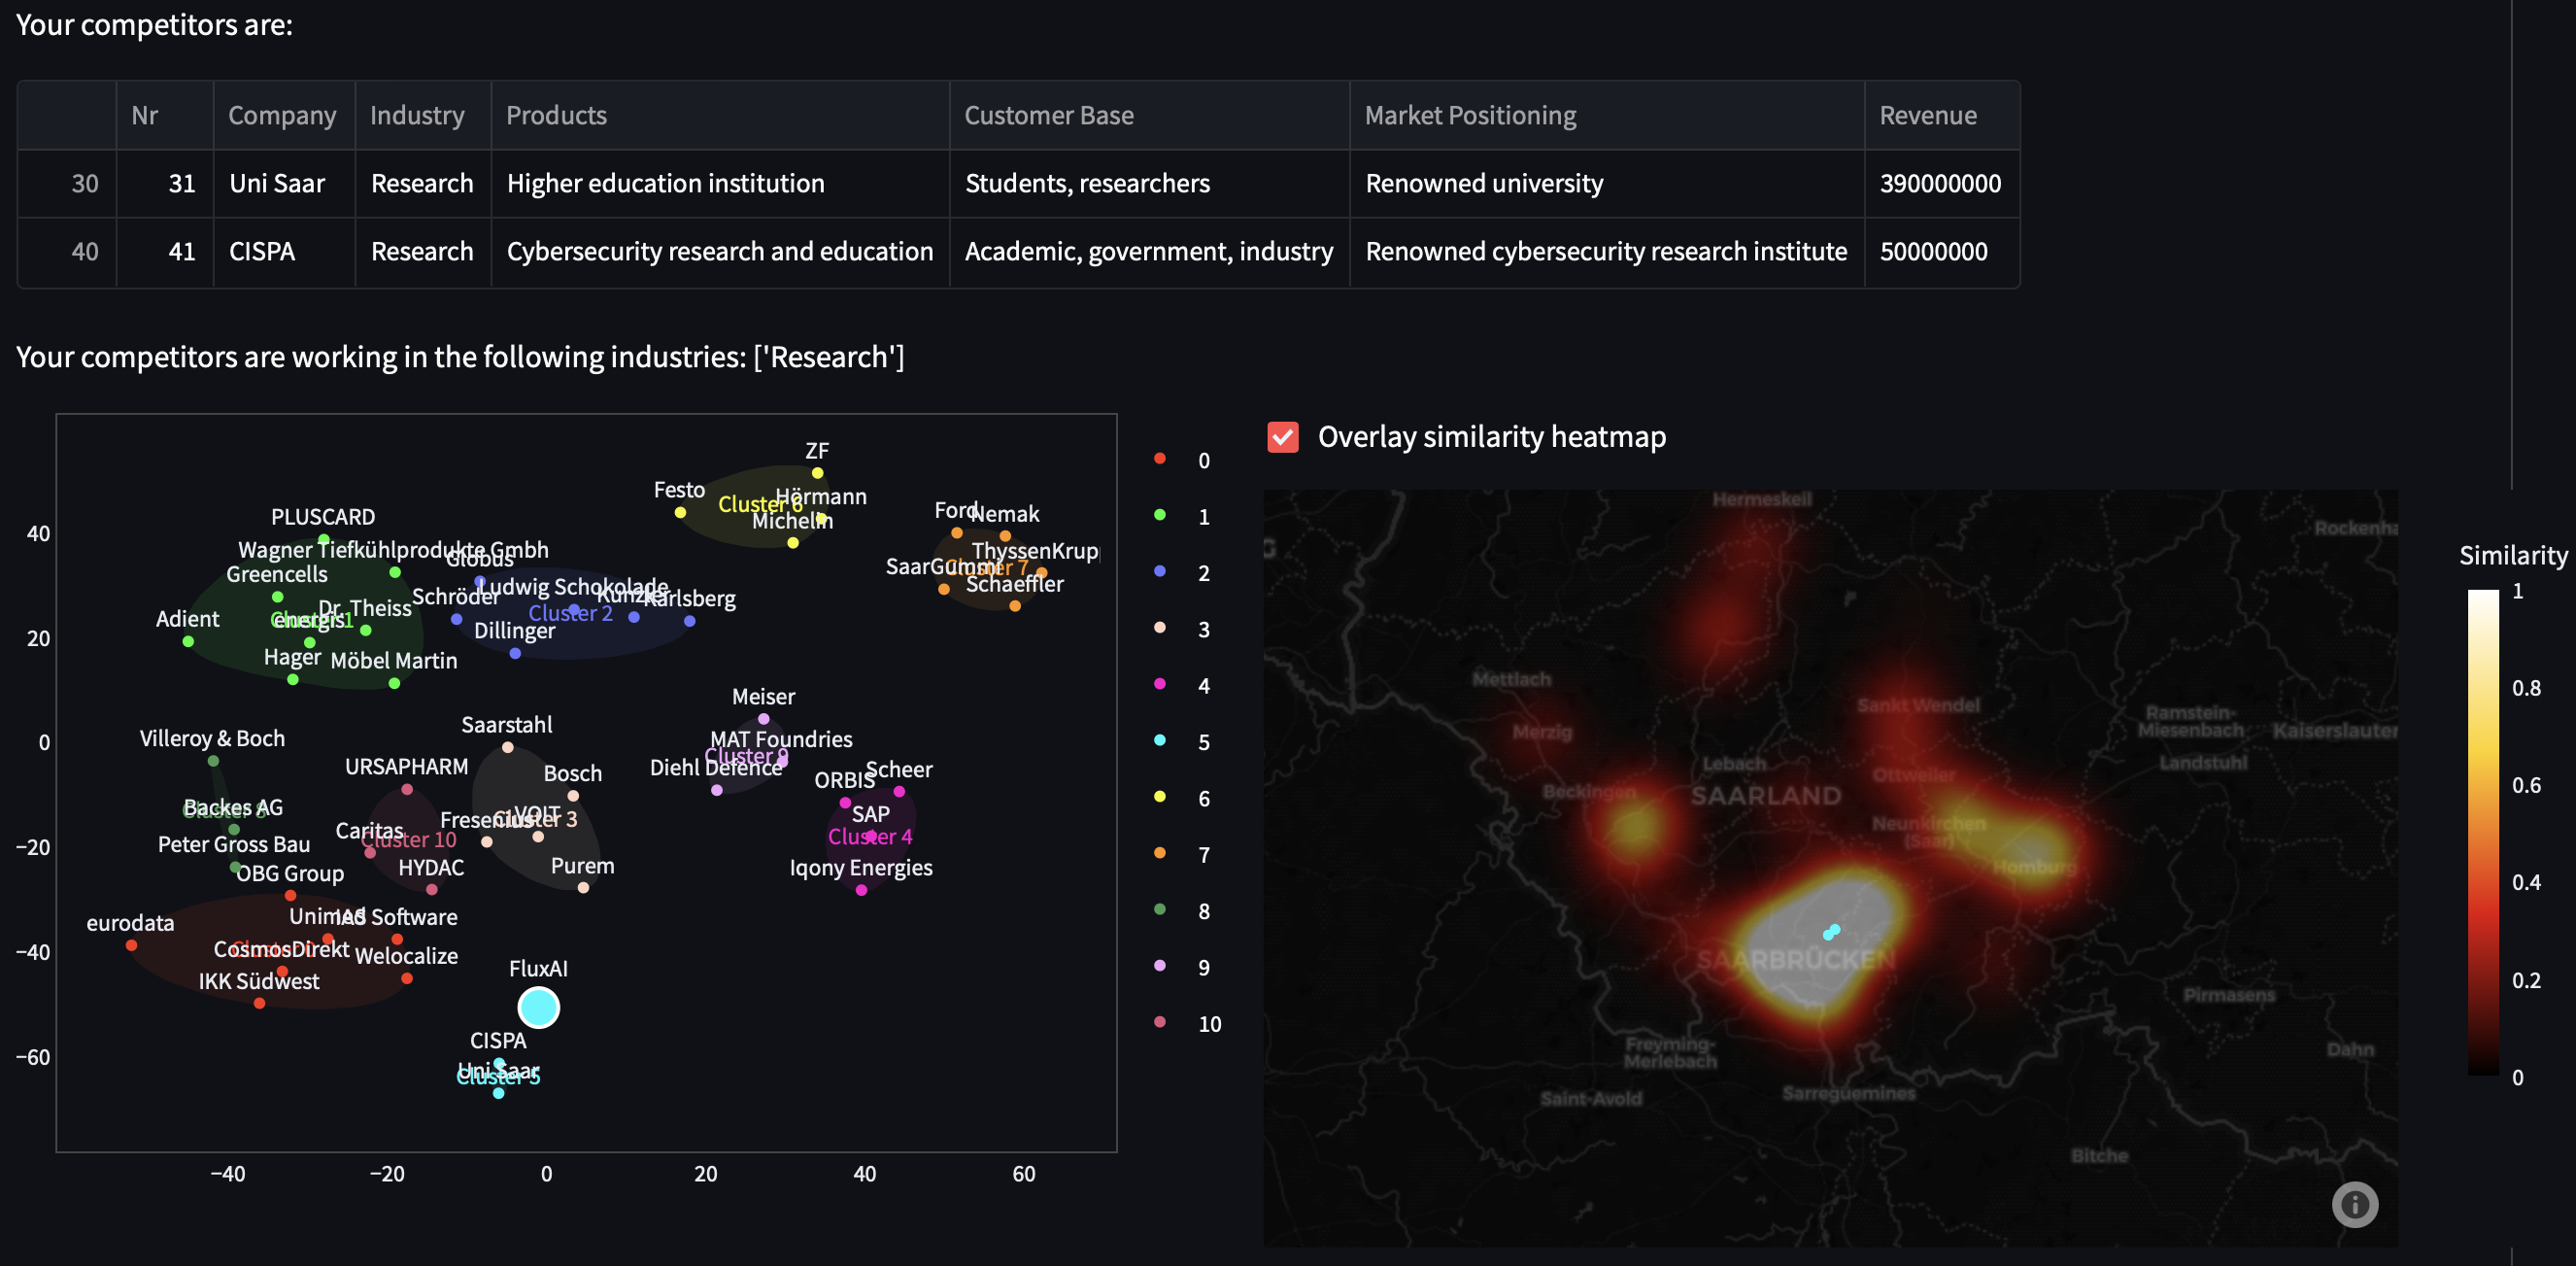
\includegraphics[width=\textwidth]{figures/location_recommendation_output.png}
   		\caption{Output of the location recommendation feature of our user-interface.}
   		\label{fig:location-recommendation-output}
   	\end{subfigure}
   \end{figure}
   
   %\subsection{Fostering Business Clusters through Location Recommendations}
   To give location recommendations for companies seeking to establish new sites in the region of interest, we utilize parts of our clustering pipeline. Given the novel company's description, we compute an embedding and apply dimensionality reduction. We then assign the data point to a cluster and compute which company within the cluster is most similar to the novel company.
   Given the novel company's cluster label, the location recommendation is to establish a new site nearby the most similar company within the cluster. Thus, our location recommendations support the geographical concentration of companies acting in the same market segment, which helps to foster business clusters.
   
   Our user-interface offers a dedicated tab for location recommendations. Users can provide their company's name and description in text boxes. Additionally, they can specify their company's industry, products, customer base, market position, and revenue. After clicking "Submit", users are shown the output depicted in figure \ref{fig:location-recommendation-output}. The table at the top shows the names and features of the companies in the cluster to which the user's company was assigned. The scatter plot at the bottom left shows the clustered data points, where the point of the user's company is highlighted. Lastly, the map at the bottom right displays the location of the novel company's cluster members and the distances between them. The user can also overlay a heatmap that shows the similarity between his company and all other companies in the dataset.
   
   \section{Results}
   To build a dataset of company descriptions, we extracted the descriptions of $50$ of the largest companies in Saarland, which are listed in the appendix \ref{sec:appendix-companies}.
   For the experimental evaluation, we conducted the data collection manually. However, in the future, we aim to create an HTML scraper to scale our approach to larger regions. To test our location recommendation feature, we created company descriptions using GPT-4 \cite{chatgpt}.
   Additionally, we evaluate the impact of providing additional features to the clustering pipeline, for which we also gathered the features industry, products, customer base, market positioning, and revenue of each company. 
   We utilize the popular pre-trained sentence transformer model "all-MiniLM-L6-v2"~\cite{sentence-transformer-model} to compute sentence embeddings for each description.  
   
   \begin{figure}[H]
   	\centering
   	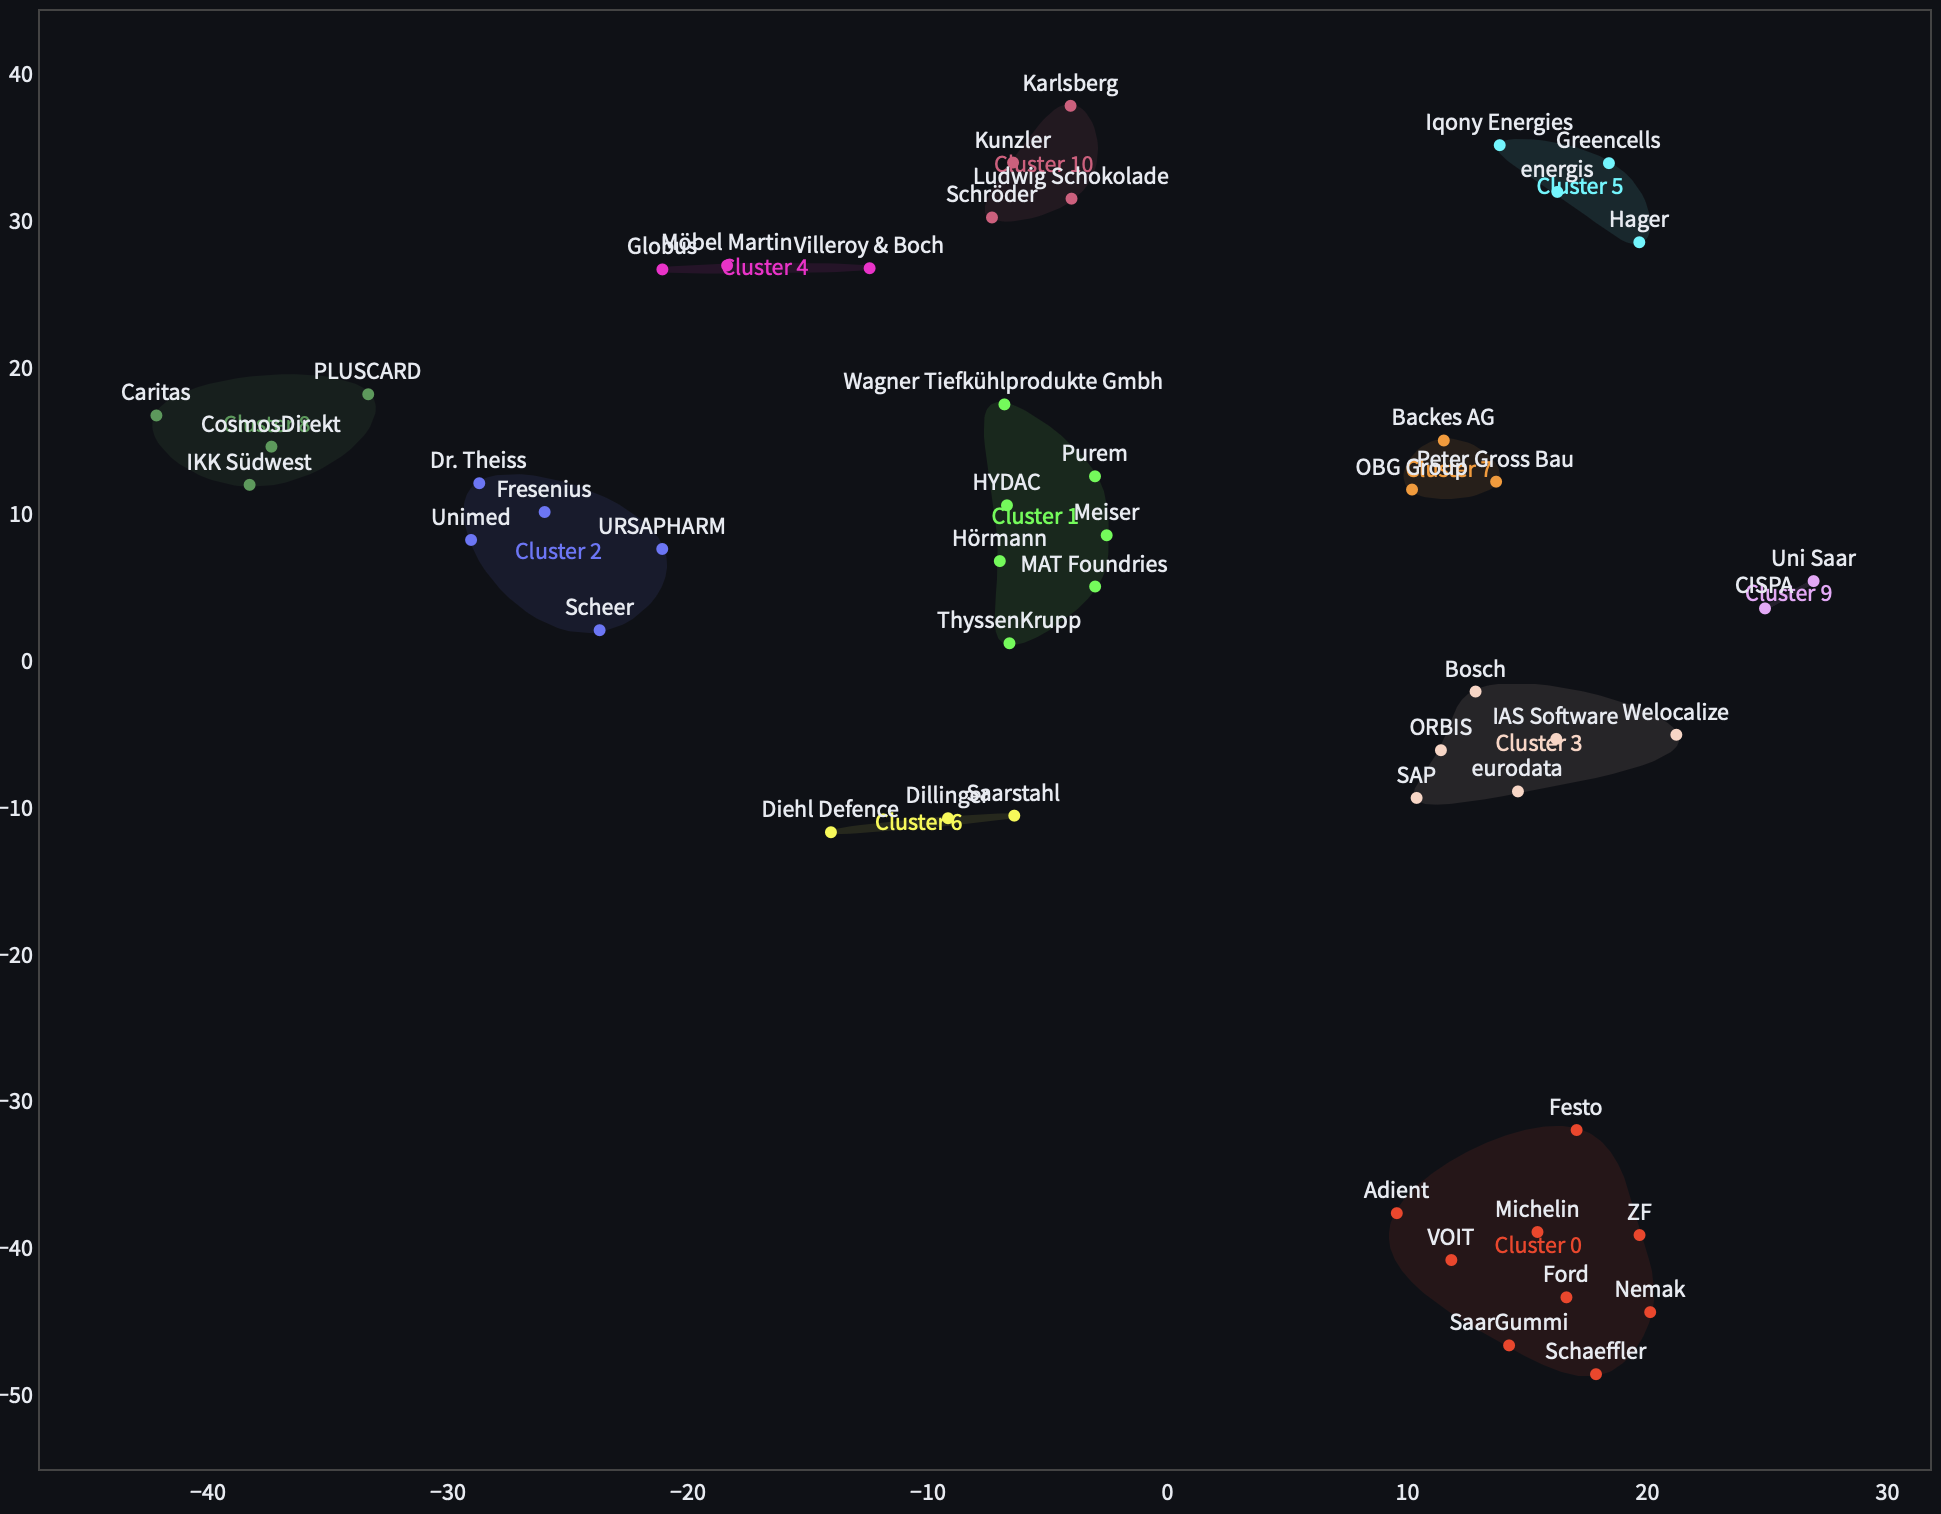
\includegraphics[width=0.5\textwidth]{figures/clustering_results.png}
   	\caption{Clustering of company descriptions using t-SNE and Agglomerative clustering. The company descriptions and industries were used as features.}
   	\label{fig:t-sne-agglomerative}
   \end{figure}
   
   We will now investigate the results of our clustering and location recommendation system. Besides the company descriptions, we used the companies' industry as an additional feature since this yielded the most concise clustering. Figure \ref{fig:t-sne-agglomerative} displays the resulting clustered data points.
   To evaluate  the clustering of our pipeline, we will compare the found clusters to those identified in \cite{saarlandeco2} (Table 4, p. 1226):
   \textit{Coal and mining industries}: With the decline of coal mining in recent years, there are no more coal mines in Saarland. Accordingly, no such companies are present in our dataset.    
   \textit{Metal industry}: Covered by cluster 1 (light green) and cluster 6 (yellow), which contain steel producers like SaarStahl and Dillinger and companies offering steel products like Hörmann, a producer of various types of doors.    
   \textit{Automobile industry}: Saarland's large automobile market segment is covered by cluster 0 (red), including companies like Ford, ZF, and Michelin.    
   \textit{Energy}: Cluster 5 (light blue) comprises the energy provider energis and the energy service providers Iqony Energies and Greencells, representing the energy market segment.    
   \textit{Information and communication technology}: The IT products and IT consulting market segment, to which companies like SAP, ORBIS, and eurodata belong, is covered by cluster 3 (beige).    
   \textit{Biotechnology and nanotechnology}: Covered by cluster 2 (dark blue), with members such as Fresenius, which produces dialysis machines, and USRAPHAM, which manufactures medicine.        
   One can see that the results of our pipeline agree with the general sectors identified by \cite{saarlandeco2}. However, our approach did lead to more fine-grained separation. Additionally, we identified sectors not covered in their work, such as cluster 7 (orange), which represents the construction work market segment, and cluster 10 (pink), which represents the food production market segment.
   
   To test our location recommendation system, we generated descriptions for three fictional German companies with vastly different characteristics:
   \textit{FluxAI}: A young artificial intelligence start-up with ambitious goals of revolutionizing healthcare, finance, energy, and transportation.    
   \textit{ABC Auto}: A well-established automotive manufacturer offering a wide range of cars focusing on sustainability.    
   \textit{PanzerTech}: A weapons manufacturer with a wide spectrum of products, from armored vehicles to cybersecurity solutions.       
   For FluxAI, our system recommends placing the new site close to CISPA, which is sensible since CISPA is a world leader in information security research, including artificial intelligence, and thus knowledge transfer between both companies could be highly beneficial. 
   For ABC Auto, the location recommendation is to establish a new site close to VOIT, which specializes in manufacturing car components with a focus on hybrid and electric cars. Thus, placing ABC Auto near VOIT would allow ABC Auto to source parts for its hybrid and electric cars from a company nearby, leading to a more robust supply chain.
   Lastly, our system recommends placing PanzerTech's new site close to Diehl Defence, corresponding to the only weapons manufacturer in our dataset. Hence, this shows that our system does not need many samples from each market segment to give reasonable location recommendations.   
   We conclude that our location recommendation system can reliably identify companies in our dataset with similar characteristics to companies seeking to establish sites in Saarland and thus can be used to foster the development of business clusters.
   
   \section{Conclusion}
   In this work, we demonstrated how language models and clustering algorithms could be combined to identify market segments and give location recommendations for novel companies such that business clusters are fostered.
   
   We represented companies by their public descriptions, which allowed us to leverage state-of-the-art language models to transform the highly informative text data into embeddings. Further, our methods enabled straightforwardly including other company attributes. Given the embeddings, we applied a clustering algorithm to infer potential market segments.
   To make location recommendations, we passed the descriptions and features of novel companies to our clustering pipeline and recommended establishing new sites next to the most similar companies in our dataset.
   
   A qualitative evaluation of our methods has shown that they can reliably cluster similar companies, which allowed us to infer market segments in Saarland. Further, our location recommendation system demonstrated its capability of identifying similar companies, given the description of a new company.
   
   To allow end-users to leverage our methods, we implemented a user-friendly interface with many functionalities, such as visualizing the clustered data points, showing the location of companies, and giving detailed and interpretable location recommendations.
   
   A promising opportunity for future work would be fine-tuning our language models using text data from the business sector since it might lead to more expressive embeddings. To achieve this efficiently, an automated aggregation system could be developed. As we rely on public websites, such a system could be easily implemented without relying on 3rd party services.
   
   To this end, we have demonstrated the feasibility and potential of applying language models to economic analysis.
    
    \bibliographystyle{IEEEtran}
	\bibliography{bibliography}
	
	\newpage
	\section{Appendix}
	
	\subsection{Link to Code}
	\url{https://github.com/NicolaMueller42/data_science_project}
	
	\subsection{Companies in our Dataset}
	\label{sec:appendix-companies}
	
	We list the $50$ Saarland companies in our dataset:
	\begin{multicols}{4} \begin{itemize}
	   		\item ZF
	   		\item Saarstahl
	   		\item Dillinger
	   		\item Bosch
	   		\item Festo
	   		\item Ford
	   		\item Schaeffler
	   		\item Fresenius
	   		\item Wagner
	   		\item \footnotesize Villery\&Boch \normalsize
	   		\item Michelin
	   		\item \scriptsize ThyssenKrupp \normalsize
	   		\item Hager
	   		\item Purem
	   		\item \small SaarGummi \normalsize
	   		\item VOIT
	   		\item Meiser
	   		\item SAP
	   		\item Nemak
	   		\item Peter Gross Bau
	   		\item OBG Group
	   		\item \scriptsize URSAPHARM \normalsize
	   		\item Hörmann
	   		\item Kunzler
	   		\item Diehl \\Defence
	   		\item HYDAC
	   		\item Backes AG
	   		\item Karlsberg
	   		\item Globus
	   		\item Caritas
	   		\item Uni Saar
	   		\item Welocalize
	   		\item Möbel Martin
	   		\item IKK Südwest
	   		\item Dr. Theiss
	   		\item Unimed
	   		\item CosmosDirekt
	   		\item ORBIS
	   		\item eurodata
	   		\item energis
	   		\item CISPA
	   		\item Greencells
	   		\item Scheer
	   		\item Iqony Energies
	   		\item PLUSCARD
	   		\item IAS Software
	   		\item Ludwig Schokolade
	   		\item MAT Foundries
	   		\item Adient
	   		\item Schröder
	\end{itemize}\end{multicols}
    
\end{document}